\chapter{Стабилизация с идеальным дифференцирующим звеном}
\label{ch:chap1}
\newcommand\tab[1][1cm]{\hspace*{#1}}

\ExplSyntaxOn
\clist_new:N \l_feq_vector_clist
\NewDocumentCommand{\feqvector}{O{\\}mO{b}}{
  \clist_set:Nn \l_feq_vector_clist {#2} % Set the list
  \begin{#3matrix}
  \clist_use:Nn \l_feq_vector_clist {#1} % show it with separator from #1 (\\)
  \end{#3matrix}
}
\ExplSyntaxOff


Перед нами объект управления 2-го порядка, заданный дифференциальным уравнением:
$$
a_2\ddot{y} + a_1\dot{y} + a_0y = u
$$

Придумаем такие $a_2,a_1,a_0$, чтобы система содержала хотя бы один неустойчивый полис.

Воспользуемся для этого старой доброй - теоремой Виета:
$$
\begin{cases}
  \lambda_1\lambda_2 = \frac{a_0}{a_2} \\
  \lambda_1 + \lambda_2 = - \frac{a_1}{a_2} 
\end{cases}
$$
Допустим\dots

$$
\begin{cases}
  \lambda_1\lambda_2 = \frac{-3}{1} \\
  \lambda_1 + \lambda_2 = - \frac{-2}{1} 
\end{cases}
$$
Тогда получаем следующие коэффициенты:
$$
\begin{aligned}
  \lambda_1 = 3 \\
  \lambda_2 = -1, \\
  a_0 = -3, \\
  a_1 = -2, \\
  a_2 = 1
\end{aligned}
$$

\begin{figure}[ht]
  \centering
  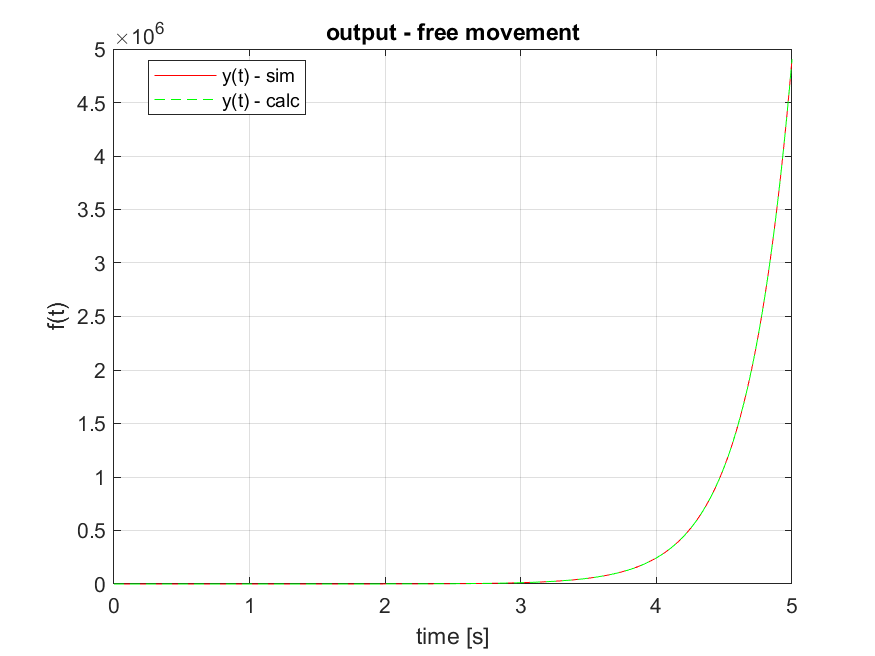
\includegraphics[width=0.6\textwidth]{output_task1_exp1.png}
\caption{Симуляция - свободное движение, $\dot{y}(0)=3, y(0) = 3$}
\end{figure}


\newpage
В этом случае мы получим следующее аналитическое выражение, уже учитывая прошлые начальные условия:
$$
y_{open}(t) = 1.5(e^{-t} + e^{3t})
$$
Как можно заметить по графику выше, результаты симуляции и аналитический расчётов совпадут.
\newpage
Рассмотрим ПД-регулятор:
$$
u = k_0y + k_1\dot{y}
$$

Получим следующую схему для нашей замкнутой системы с ПД-регулятором в режиме стабилизации:
\begin{figure}[ht]
  \centering
  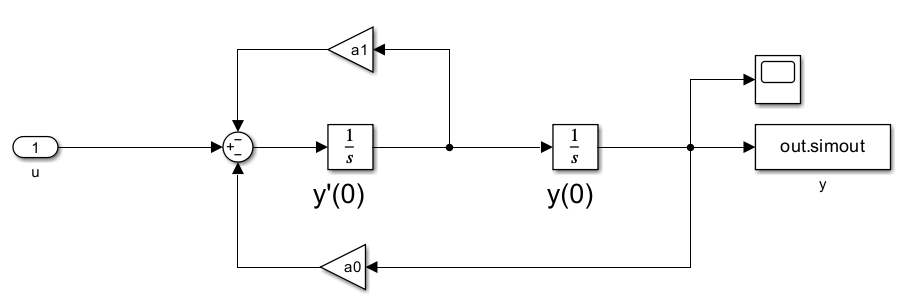
\includegraphics[width=0.8\textwidth]{scheme_system1.png}
\caption{Структурная схема - замкнутая система с ПД-регулированием}
\end{figure}

Выполним некоторые преобразования над уравнением системы, чтобы воспользоваться критерием Гурвица:
$$
  \begin{aligned}
    a_2\ddot{y} + a_1\dot{y} + a_0y = k_0y + k_1\dot{y} \\
    a_2\ddot{y} + (a_1-k_1)\dot{y} + (a_0 - k_0)y = 0 \\
    \ddot{y} + \frac{a_1-k_1}{a_2}\dot{y} + \frac{a_0 - k_0}{a_2} y = 0
  \end{aligned}
$$
Следуя критерию, получим следующие неравенства в общем виде:
$$
\begin{cases}
  \frac{a_1-k_1}{a_2} > 0, \\
  \frac{a_0 - k_0}{a_2} > 0
\end{cases}
$$
В нашем случае они чуть упростится:
$$
\begin{aligned}
  k_1 \in (-\infty, -2), \\
  k_0 \in (-\infty, -3)
\end{aligned}
$$
Возьмём конкретные значения параметра, чтобы провести моделирование, начальные условия возьмём такие же, как в прошлом опыте:
$$
k_1 = -4, k_0 = -6
$$
\begin{figure}[ht]
  \centering
  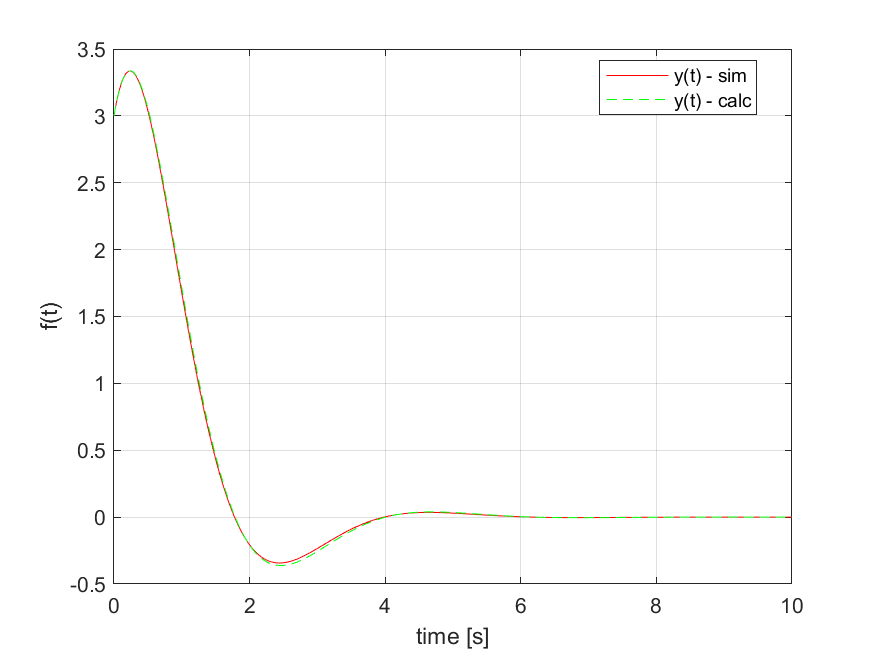
\includegraphics[width=0.8\textwidth]{output_task1_exp2.png}
\caption{Симуляция - асимпотитчески устойчивая система с ПД-регулированием}
\end{figure}

В этом случае мы получим следующее аналитическое выражение, уже учитывая прошлые начальные условия:
$$
y_{closed}(t) = e^{-t}(3cos(\sqrt{2}t) + \frac{6}{\sqrt{2}}sin(\sqrt{2}t))
$$
Как можно заметить по графику выше, результаты симуляции и аналитический расчётов также совпадают.

Сделаем промежуточные выводы: два графика выше отличаются своей устойчивостью, показывая то, 
что если мы подберём "хорошие" коэффициенты регулятора, 
то сможем получить асимпотическую устойчивость, это можно назвать неким свойством работы регулятора.

\endinput